% !TEX root=../pldi2019.tex



\section{Language}
\label{sec:language}


\subsection{Expressions}

\label{sub:expressions}
We take our host language to be a simply typed $\lambda$-calculus
extended with some basic types and \ML-style references.
The grammar in \autoref{fig:language-grammar} defines our language expressions.
Next to abstraction, application and variables,
we add constants for booleans, integers and strings.
We represent binary operations on these types by a $\star$.

The used extensions are \fixme{indicated} by the way we model tasks.
For the result of parallel tasks,
we need pairs.
An $\If{}{}{}$ expression comes in hand when defining guards.
To implement shared editors,
we will make use of references.
Creating a reference using the keyword $\Ref$ will result in a location $l$.
Locations are internal to the language and not intended to be directly manipulated by the programmer.
Dereferencing is done by using a bang,
for assigned one can use the $:=$ operator.
The unit value will be used as the result of an assignment.

\begin{figure}[h]
  \small
  \usemacro{G-Language-Compact}
  \caption{Language grammar} \label{fig:language-grammar}
\end{figure}

\label{sub:notation}
We will use double quotation marks ($\str{}$) to denote strings.
Integers are denoted by their decimal representation,
and booleans are written $\True$ and $\False$.
We will freely make use of the logic operators $\Not$, $\land$, and $\lor$,
arithmetic operators $+$, $-$, $\times$,
and the string append operator $\pp$.
Also, we will use the standard comparison operations $<$, $\le$, $\equiv$, $\not\equiv$, $\ge$, and $>$
as builtins.
Only when referring to operators in general we will use $\star$,
like in evaluation rules.
\label{sub:abbreviations}
Also, we will use the notation $e_1; e_2$
as an abbreviation for $(\lambda x:\Unit.\ e_2)\ e_1$,
and the notation $\Let x:\tau = e_1 \In e_2$
as an abbreviation for $(\lambda x:\tau.\ e_2)\ e_1$.
In both expressions $x$ is a fresh variable.

We will embed our task language into this basic language.
This means we can use all the power of the host language,
such as arithmetic operations and (higher order) functions,
in our task language.

\label{sub:pretasks}
The syntactic category $p$ of \emph{pretasks},
is further specified in \autoref{fig:task-grammar}.
A pretask $p$ is a task \emph{in making},
just as an expression is a value in making.
In the next subsections we will discuss each category of pretasks:
editors, steps and combinations.
As a general rule of thumb,
we will use open symbols ($\Edit, \Enter, \Next, \Xor$) where user input is required,
and closed symbols ($\Update, \Then, \Or$) where language constructs itself can make decisions.

\begin{figure}[h]
  \small
  \usemacro{G-Pretasks-Compact}
  \caption{Task grammar} \label{fig:task-grammar}
\end{figure}



\paragraph{Typing}

% Typing of our expressions $e$ is as to be expected.
% and won't be given in this document.
\Autoref{fig:type-grammar} shows the grammar of types used by \TOPHAT.
It contains standard types like functions, pairs, and unit,
some basic types, and a type for references.
The one difference with respect to standard work,
is the addition of a type for tasks: $\Task \tau$.

\begin{figure}[h]
  \small
  \usemacro{G-Types-Compact}
  \caption{Type grammar} \label{fig:type-grammar}
\end{figure}

Typing rules are of the form $\RelationT$,
which we read as \enquote{in environment $\Gamma$ and store typings $\Sigma$, expression $e$ has type $\tau$}.
The rules typing pretasks are given in \autoref{fig:typing-rules}.
The remaining constructs of our host language are standard,
therefore the typing rules for this part of our language are presented in the appendix.

\begin{figure}[h]
  \small
  \begin{mathpar}
    \boxed{\RelationT} \\
    \userule{T-Edit} \quad
    \userule{T-Enter} \quad
    \userule{T-Update} \\
    \userule{T-Then} \quad
    \userule{T-Next} \\
    \userule{T-And} \\
    \userule{T-Or} \quad
    \userule{T-Xor}\\
    \userule{T-Appoint} \quad
    \userule{T-Fail}
  \end{mathpar}
  \caption{Typing rules} \label{fig:typing-rules}
\end{figure}



\subsection{Editors}

In the introduction we claimed to create a language to model \emph{interactive} workflows.
By interaction we mean \emph{communication with people using the developed system}.
These end users should be able to enter information into the system,
change it, clear it, reenter it, etc.
To do this, we introduce the concept of an \emph{editor}.

Editors may or may not contain a current value.
When an editor has a value, it can be \emph{changed} or it can be \emph{emptied}.
When it is empty, a value can be \emph{filled}.
This is depicted as a state diagram in \autoref{fig:editor-state} below.

\begin{figure}[h]
  \centering
  \includegraphics[width=\columnwidth,page=3]{figures/drawings-crop.pdf}
  \caption{
    Possible states of an editor and its transitions.
    Note that shared editors cannot be cleared.
  }
  \label{fig:editor-state}
\end{figure}

One can consider editors as an abstraction over widgets in a \GUI,
form fields on a webpage,
or even sensors plugged into the system.
Take for example an entry for text.
Users can enter a string, change it, remove it, enter another string, and so on.
With editors we try to capture this \emph{constantly changing nature of user input}.
Also, because editors are \emph{typed},
they are only allowed to contain information of the right format.

How exactly information is entered is not of great importance.
This could be an input field for a string,
a switch for a boolean,
a spin box for an angle,
or even a map with a pin for a location.
% \Autoref{fig:editor-examples} depicts these examples.
\todo{Add figure with widget examples or not?}
In it's most banal form,
an editor is a line of text entered at a terminal and parsed to match
a string, boolean, angle or location value.



\paragraph{Valued and unvalued editors $(\Edit e, \Enter \tau)$}

At the core,
an editor is a container holding a value
or holding nothing.
Valued editors contain an expression $e$.
Therefore they inherit the type of $e$,
but embedded in the container type $\Task$.
This is expressed by the typing rule for valued editors \refrule{T-Edit}.

Unvalued editors do not have a value,
and therefore do not wrap an expression.
Because we strive to a fully typed system,
we have two options to type unvalued editors:
\begin{enumerate*}
  \item let the unvalued editor have a polymorphic type;
  \item annotate unvalued editors with a type and use that. \label{itm:annotate}
\end{enumerate*}

The first option sounds appealing.
However, consider the following use case.
We start with an editor containing the value two: $\Edit 2$.
The user can change this value, as long as it is an integer,
for example to five: $\Edit 5$.
Clearing the value results in an unvalued editor: $\Enter$.
Now, are we allowed to enter a value of some other type?
That is, can we now enter a string?
This would change the type of the editor
and violate the preservation theorem proved in \autoref{sub:preservation}!
Therefore,
we need to keep track of the type of values that can be entered into an unvalued editor
and we choose option (\ref{itm:annotate}).
The typing rule for valued editors can be found in \refrule{T-Enter}.

% Some examples of editors expressible in our language:
% \begin{itemize}
%   \item $\Edit 2$ is a valued editor which contains the integer value $2$.
%   \item $\Enter \String$ is an unvalued editor,
%     waiting for users to enter some string.
%   \item $\Edit ((\lambda x . x)\ 5)$ is a valued editor which,
%     after evaluation, will contain the value $5$.
%     (We will discuss evaluation of editors in the next section.)
% \end{itemize}


\paragraph{Shared editors $(\Update e)$}

\fixme{Write section on shared editors}


\paragraph{Fail $(\Fail)$}

\fixme{Write section on fail}


\subsection{Composition}


% In the previous section we have set up our interaction model of inputs and actions,
% we defined our interactive component, the editor,
% and introduced the infinitely failing task.
Now that we have the core part of an interactive workflow,
namely editors,
we can continue with ways to compose multiple tasks.
Combining tasks can be done in two ways:
\begin{enumerate*}
  \item sequential or
  \item parallel.
\end{enumerate*}
For parallel composition we distinguish two kinds:
\begin{enumerate*}[(a)]
  \item pairing two tasks (\emph{and}-parallel); and
  \item choosing between two tasks (\emph{or}-parallel).
\end{enumerate*}
In this subsection we start with sequential composition.
The next two subsections are about pairing and choosing.



\paragraph{System and user step $(e_1 \Then e_2, e_1 \Next e_2)$}

One might think that the best way to sequence tasks is by just following one task with another:
do this, then do that, then that, etc.
However, we like the continuation to depend on the value produced by the preceding task.
This way, we can use this information to precisely specify how to continue with work.
This is done by a \emph{step}.
We define a step from one task to another as
\begin{quote}
  a calculation which returns the next task to proceed with.
\end{quote}

To accomplish this,
we take continuations to be \emph{functions}.
These are just normal functions from our host language which,
when evaluated, result in something of type $\Task$.
Therefore,
we extend our pretasks $p$ with a sequence construct $\Then$.

The accompanied typing rule is \refrule{T-Then}.
Note that typing ensures us that the left hand side $e_1$ will be a task delivering a value of type $\tau_1$.
The right hand side $e_2$ then, will use this value of type $\tau_1$,
and calculate a new task of type $\Task \tau_2$,
holding a value of (possibly another) type $\tau_2$.



\paragraph{Parallel $(e_1 \And e_2)$}

\fixme{Write section on parallel}



\paragraph{System and user choice $(e_1 \Or e_2, e_1 \Xor e_2)$}

\fixme{Write section on choice}



\subsection{Users}

\paragraph{Appoint $(u \At e)$}

\fixme{Write section on appointing users}
\begin{itemize*}
  \item How to create users?
  \item What is their type?
\end{itemize*}
